\documentclass{beamer}
%\usepackage{projstyle}
\newcommand{\R}{\mathbb{R}}
\usepackage{graphicx}

\begin{document}

\title{An Introduction to Legendrian Knots}
\author{Shreyas Casturi, Ana Fishburn}
\date{28 November 2018}

\frame{\titlepage}

\section[Intro]{What are Legendrian Knots?}

\begin{frame}
    \frametitle{Contact Structures}
    \begin{definition}
    A \alert{contact structure} on $\R^3$ is a method of assigning a plane
    to every point, such that these planes satisfy certain technical conditions.
    \end{definition}

    Throughout, we will only consider the \alert{standard contact structure}, which
    twists along the $y$-axis: \\
    \begin{center}
        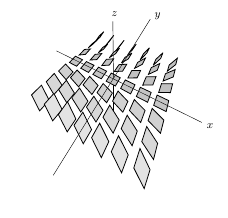
\includegraphics[height=5cm]{cStructure.png}
    \end{center}
    
\end{frame}

\begin{frame}
\frametitle{Legendrian Knots}
    \begin{definition}
    A \alert{Legendrian knot} $K$ is a smooth knot which is, at every point, parallel to the
    plane at that point given by the contact structure.
    \end{definition}

    More concretely: if $K$ is the image of $\phi : [0,1] \to \R^3$ given in coordinates by
    $t \mapsto \phi(x(t),y(t),z(t))$, then $K$
    is Legendrian if for all $t$,
    \[ z'(t) - y(t)x'(t) = 0. \]
    \begin{center}
    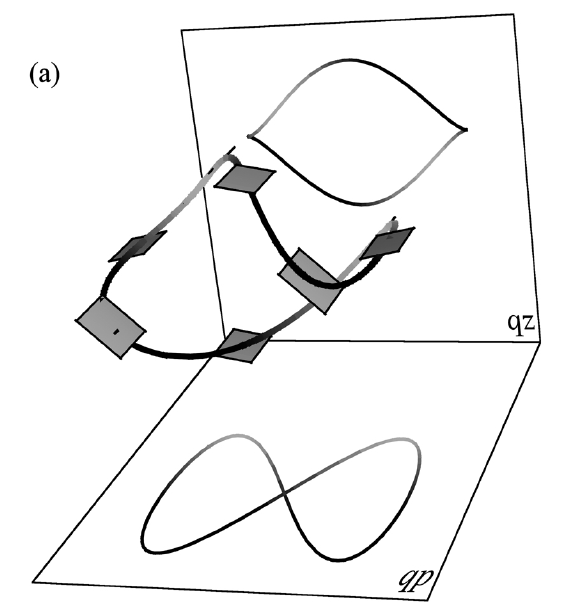
\includegraphics[height=4cm]{contactLegendrian.png}
    \end{center}

\end{frame}

\begin{frame}
    \frametitle{Equivalences of Legendrian Knots}
    Two Legendrian knots are equivalent if there is a continuous family of Legendrian
    knots between them. This is similar to the definition of smooth knot equivalence,
    only with the allowable motions restricted.

    \begin{theorem}
    If two Legendrian knots are Legendrian equivalent, then they are equivalent as smooth knots.
\end{theorem}



\end{frame}

\section[Proj]{Projections of Legendrian Knots}

\begin{frame}
    \frametitle{Projections of Legendrian Knots}
    If we want to have clear visual representations of Legendrian knots,
    we need diagrams that respect the contact structure.

    \begin{definition}
    The \alert{front projection}, denoted \alert{$\Pi(K)$}, of a Legendrian knot $K$ is the projection
    into the $xz$-plane.
    \end{definition}

    \begin{definition}
    The \alert{Lagrangian projection}, denoted \alert{$\pi(K)$}, of a Legendrian knot $K$ is the projection
    into the $xy$-plane.
    \end{definition}
    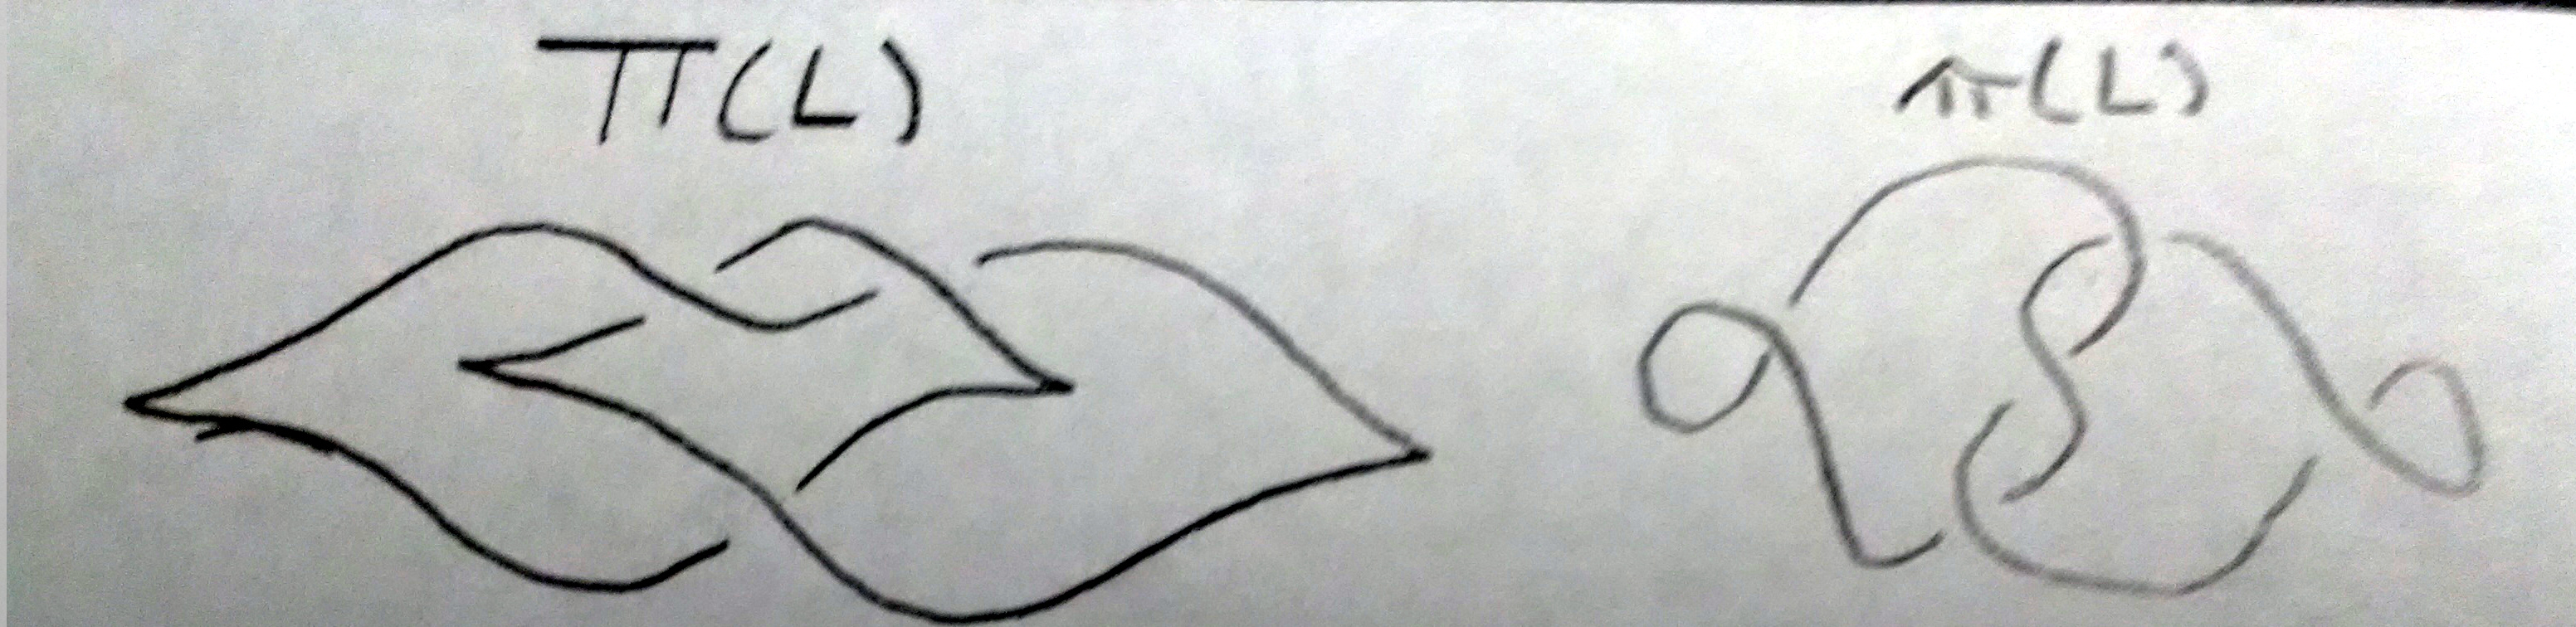
\includegraphics[height=2cm]{piPi.jpg}
\end{frame}

\begin{frame}
    \frametitle{Properties of the Front Projection}
    We solve the equation $z'(t) - y(t)x'(t) = 0$ for $y$:
    \[ y(t) = \lim_{s\to t} \frac{z'(s)}{x'(s)}. \]

    \begin{itemize}
    \item No vertical tangencies are allowed: if $z'(t) = 0$, then $x'(t)$ must also be zero.
    Instead, we allow \alert{cusps}, where the diagram makes a sharp horizontal point.
    \item At each crossing, the under strand has greater slope than the over strand.
    \end{itemize}
\end{frame}

\begin{frame}
    \frametitle{Converting Smooth Knots into Legendrian Knots}
    Taking any diagram of a smooth knot, we can get a valid front diagram for a Legendrian
    knot by the following procedure:
    \begin{itemize}
    \item Rotate the diagram around each crossing until the under strand has greater slope.
    \item Convert every vertical tangency into a cusp.
    \end{itemize}
    \begin{theorem}
        For any smooth knot $K$, there is a Legendrian knot $K'$, such that $K$ and $K'$ are
        equivalent as smooth knots.
    \end{theorem}
    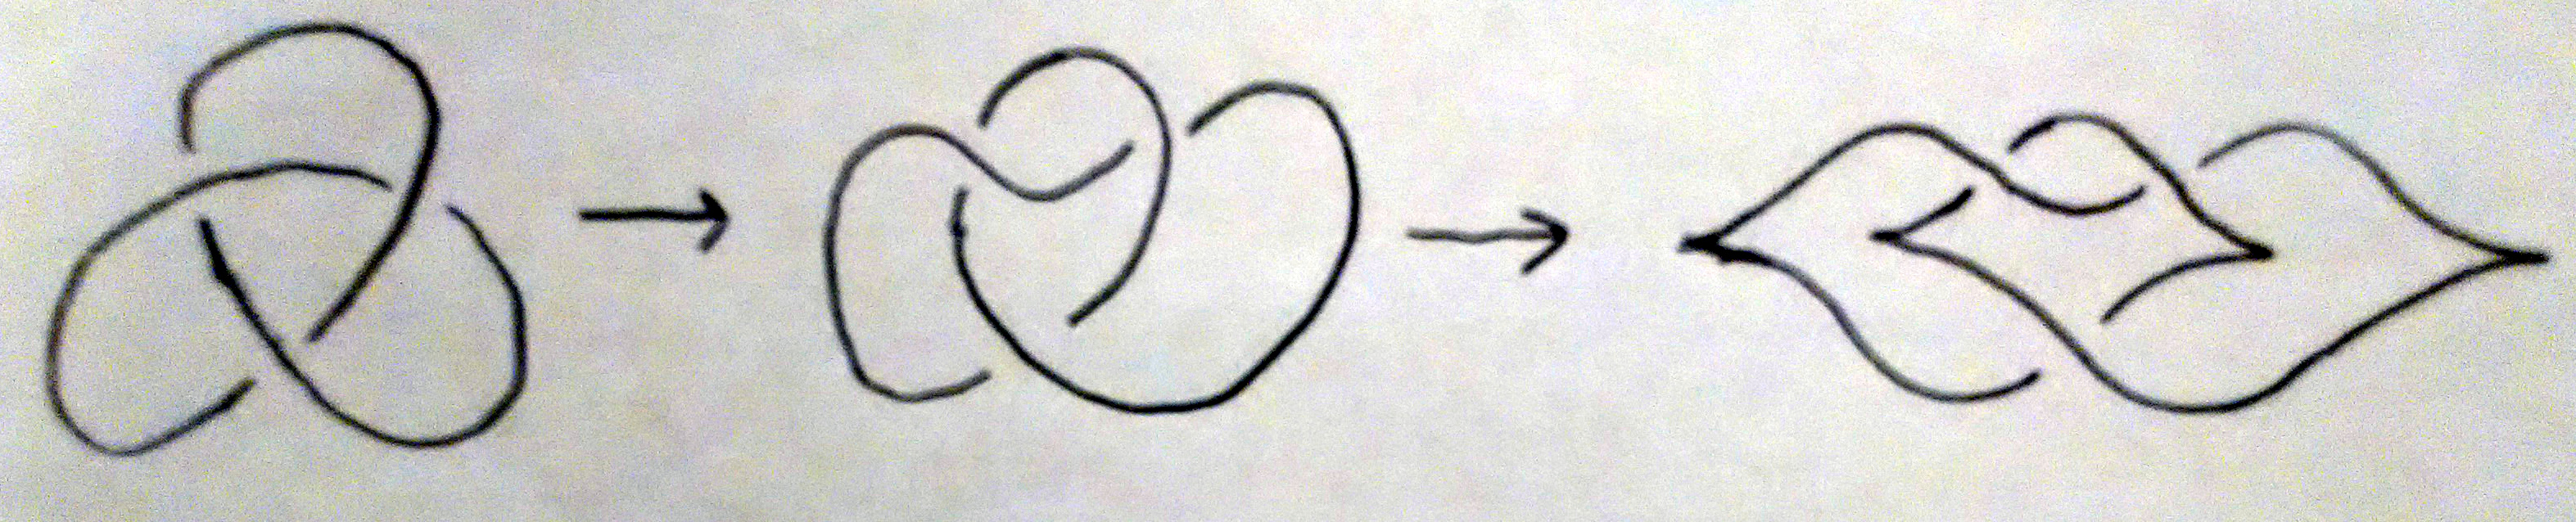
\includegraphics[height=2cm]{smoothToLegendrian.jpg}
\end{frame}

\begin{frame}
    \frametitle{Reidemeister Theorem for Front Projections}
    \begin{theorem}
        Two front projections represent equivalent Legendrian knots if and only if
        they can be related by a sequence of the following moves:
    \end{theorem}
    \begin{center}
    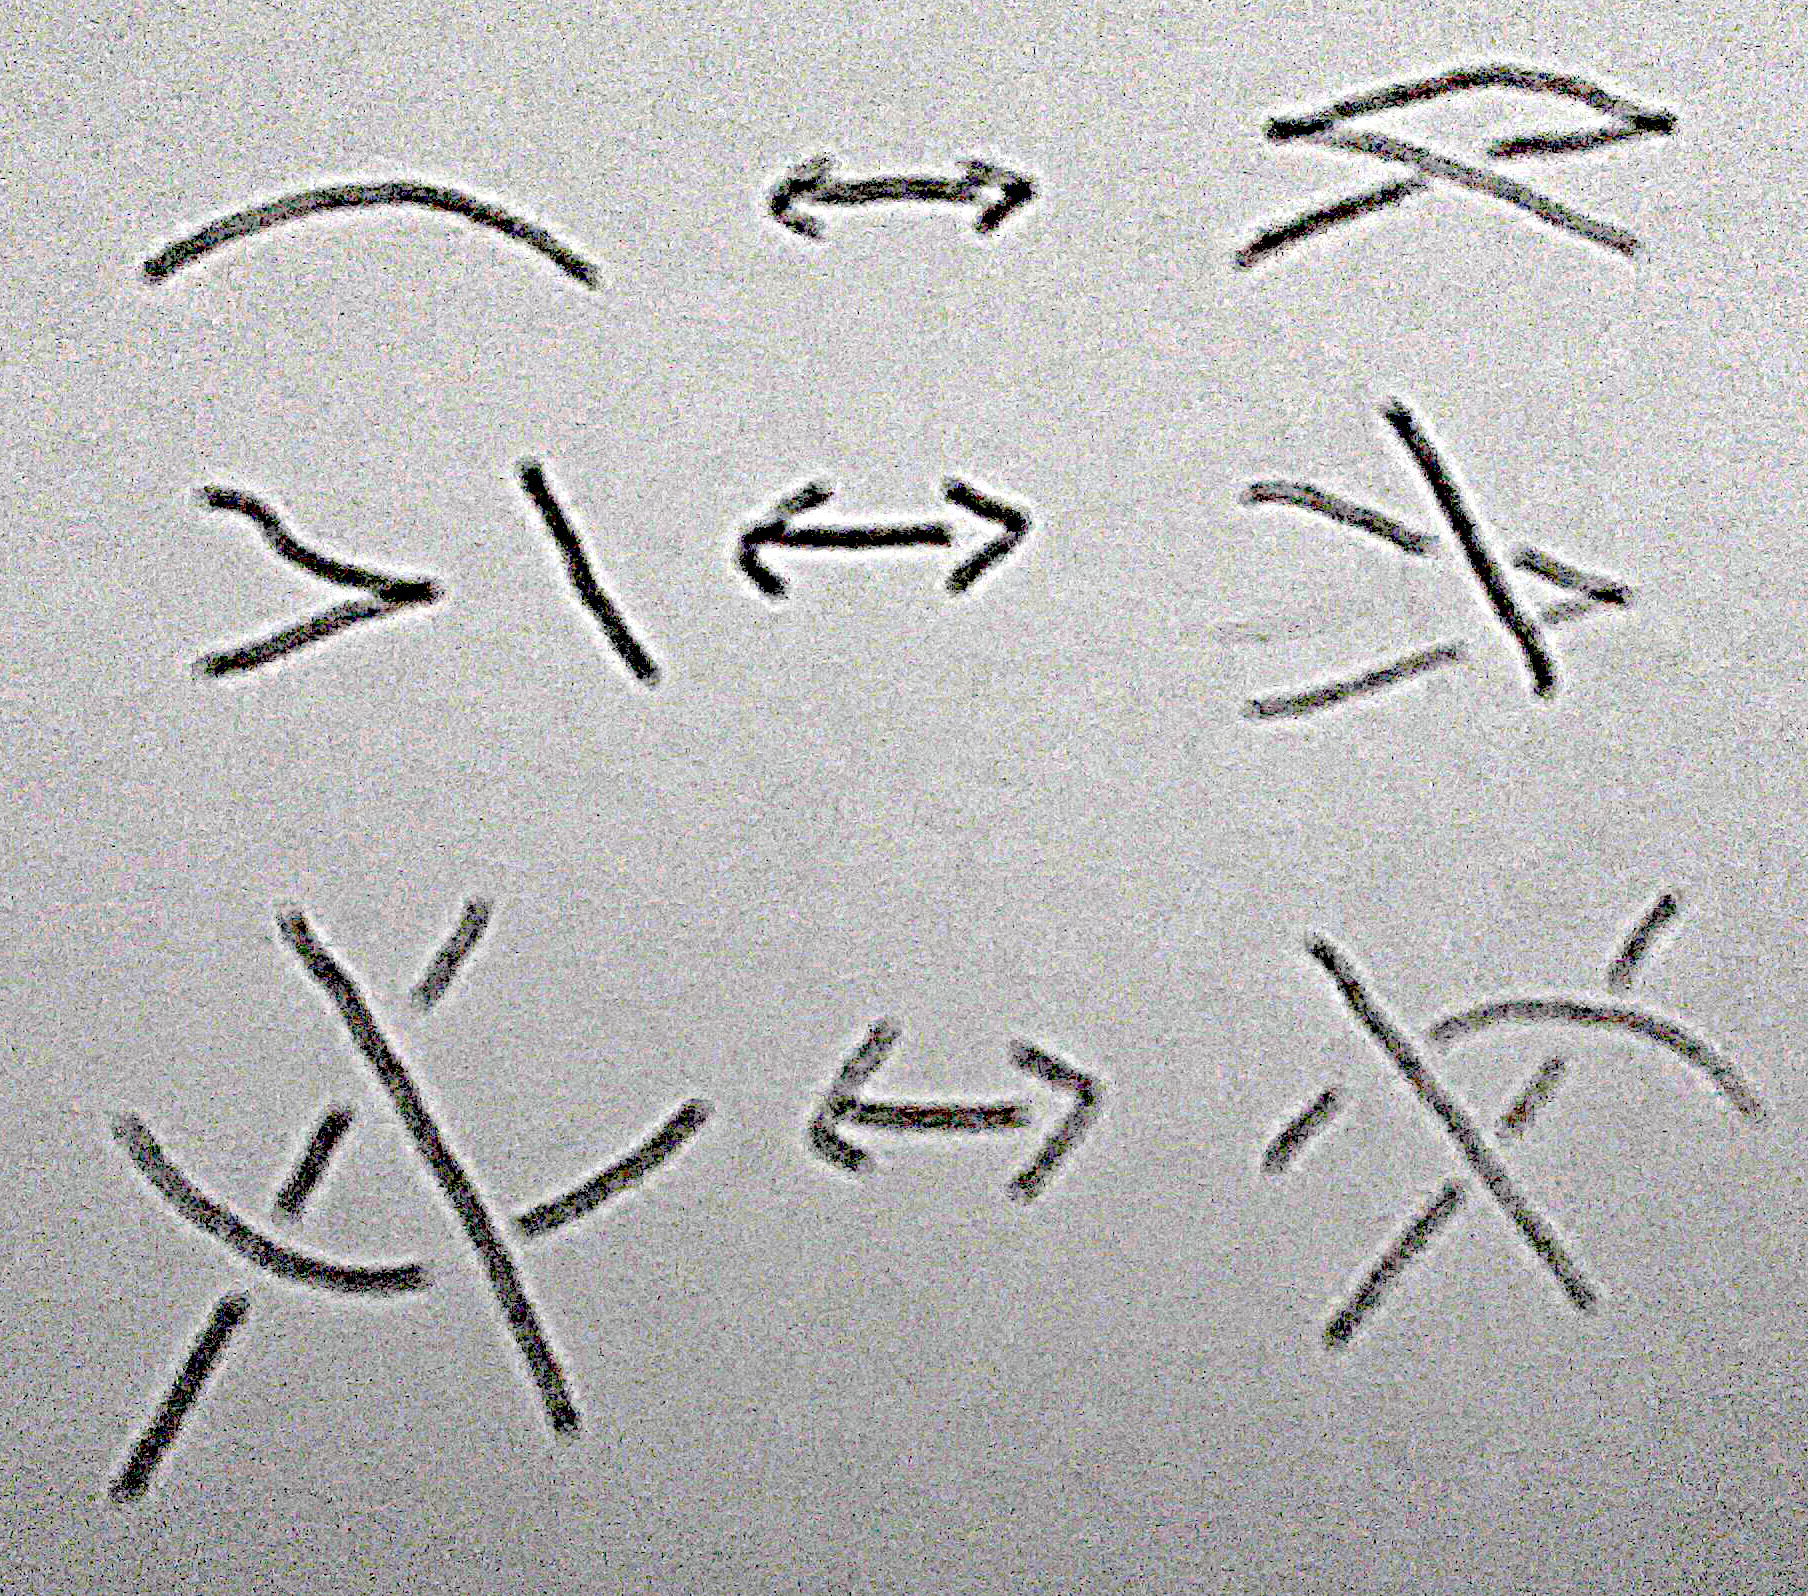
\includegraphics[height=5cm]{Redemeister.jpg}
    \end{center}
\end{frame}

\begin{frame}
\frametitle{Properties of the Lagrangian Projection}
    This time, we solve the equation $z'(t) - y(t)x'(t) = 0$ for $z$:
    \[ z(t) = z_0 + \int_0^t y(s)x'(s)\,ds, \]
    so we can always recover the $z$ coordinate (up to translation) from $\pi(K)$.

    \begin{itemize}
    \item $\int_0^1 y(s)x'(s)\,ds = 0$.
    \item $\int_{t_1}^{t_2}y(s)x'(s)\,ds \neq 0$ whenever $(x(t_1),y(t_1))=(x(t_2),y(t_2))$.
    \end{itemize}
\end{frame}

\begin{frame}
    \frametitle{Classical Invariants}
    We now consider \alert{Legendrian knot invariants}, which, similarly to smooth
    knot invariants, are functions from the set equivalence classes of Legendrian
    knots.

    There are three classical invariants we will be discussing:
    \begin{itemize}
        \item \textit{The Topological Knot Type}
        \item \textit{The Thurston-Bennequin Number}
        \item \textit{The Rotation Number}
    \end{itemize}
    \alert{NOTE}: We will consider in the following slides knots
    that have an \textit{orientation}.
\end{frame}

\begin{frame}
    \frametitle{Topological Knot Type}
    Because two Legendrian equivalent knots are automatically equivalent
    as smooth knots, we have the following invariant:
    \begin{definition}
        The \alert{topological knot type} of a Legendrian knot $L$ is $k(L)$,
        the equivalence class of all knots smoothly equivalent to $L$.
    \end{definition}
    For example the following two front diagrams give inequivalent Legendrian knots,
    because one is an unknot while the other is a figure-eight.

    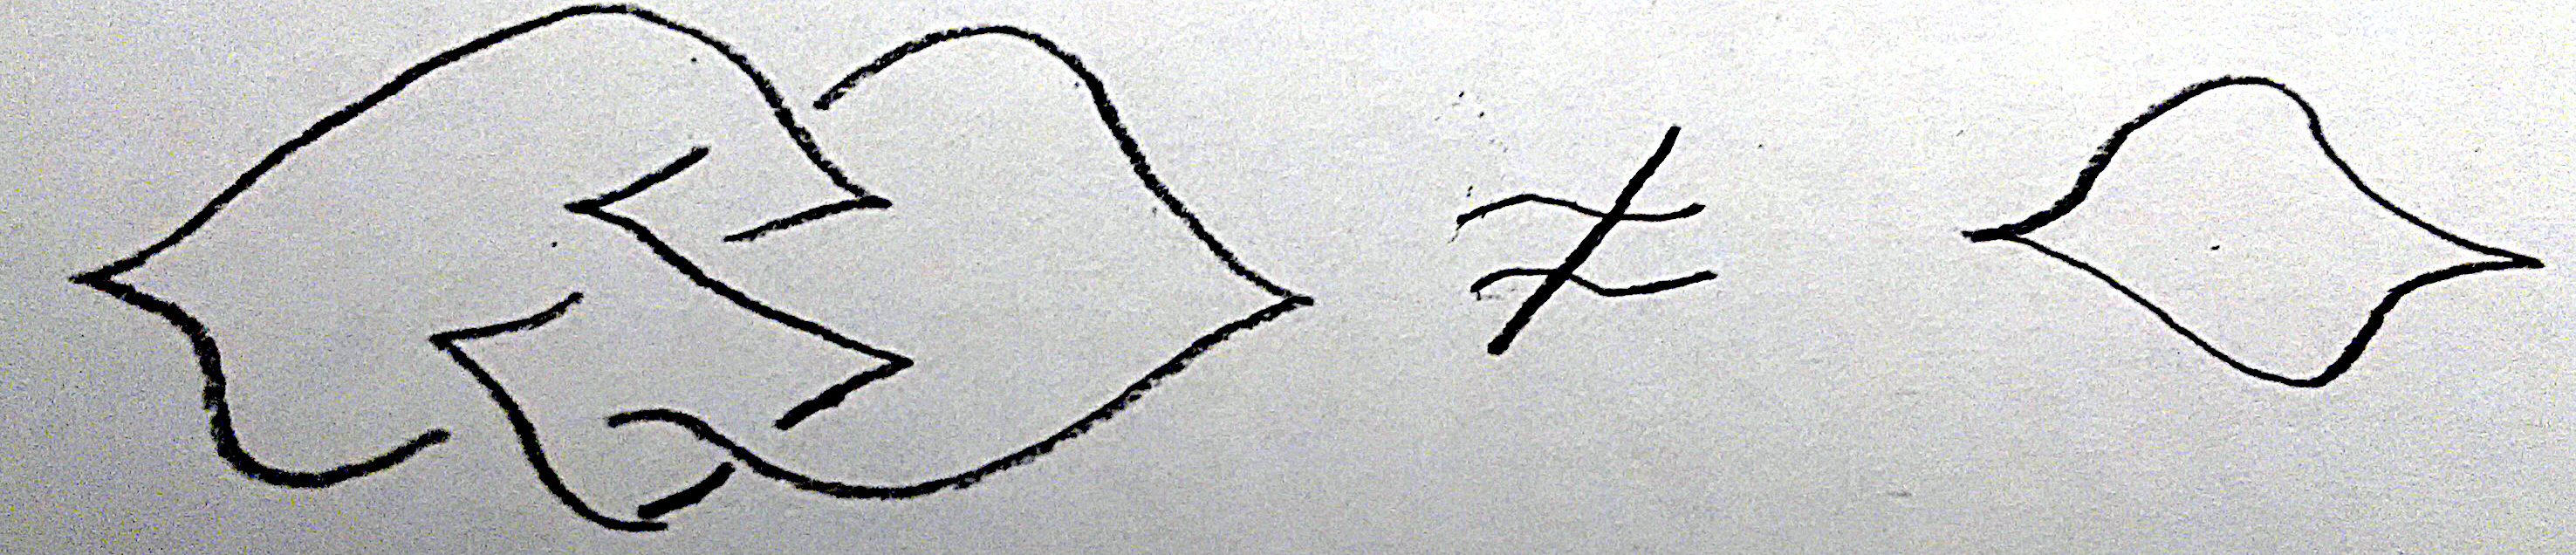
\includegraphics[height=2cm]{notEq.jpg}
\end{frame}

\begin{frame}
    \frametitle{Thurston-Bennequin Invariant}
    Geometrically, the \alert{Thurston-Bennequin number} of a Legendrian knot $L$
    measures how much the contact planes "twist" around $L$.

    We write the Thurston-Bennequin number as \alert{$tb(L)$}.
    The full definition requires some heavy geometry, so we give
    effective definitions in terms of the projections of $L$.
\end{frame}

\begin{frame}
    \frametitle{Calculating $tb(L)$ Using Front Projections}
    For a \textit{front} projection:
    \begin{itemize}
        \item There are two things we must calculate:
        \begin{itemize}
            \item The \textit{writhe} number of the knot projection.
            \item The number of \textit{cusps} the knot projection has.
        \end{itemize}
    \end{itemize}
    The formula for a front projection is
    \[tb(L) = writhe(\Pi(L)) - \frac{1}{2}(cusps).\]
    \begin{center}
    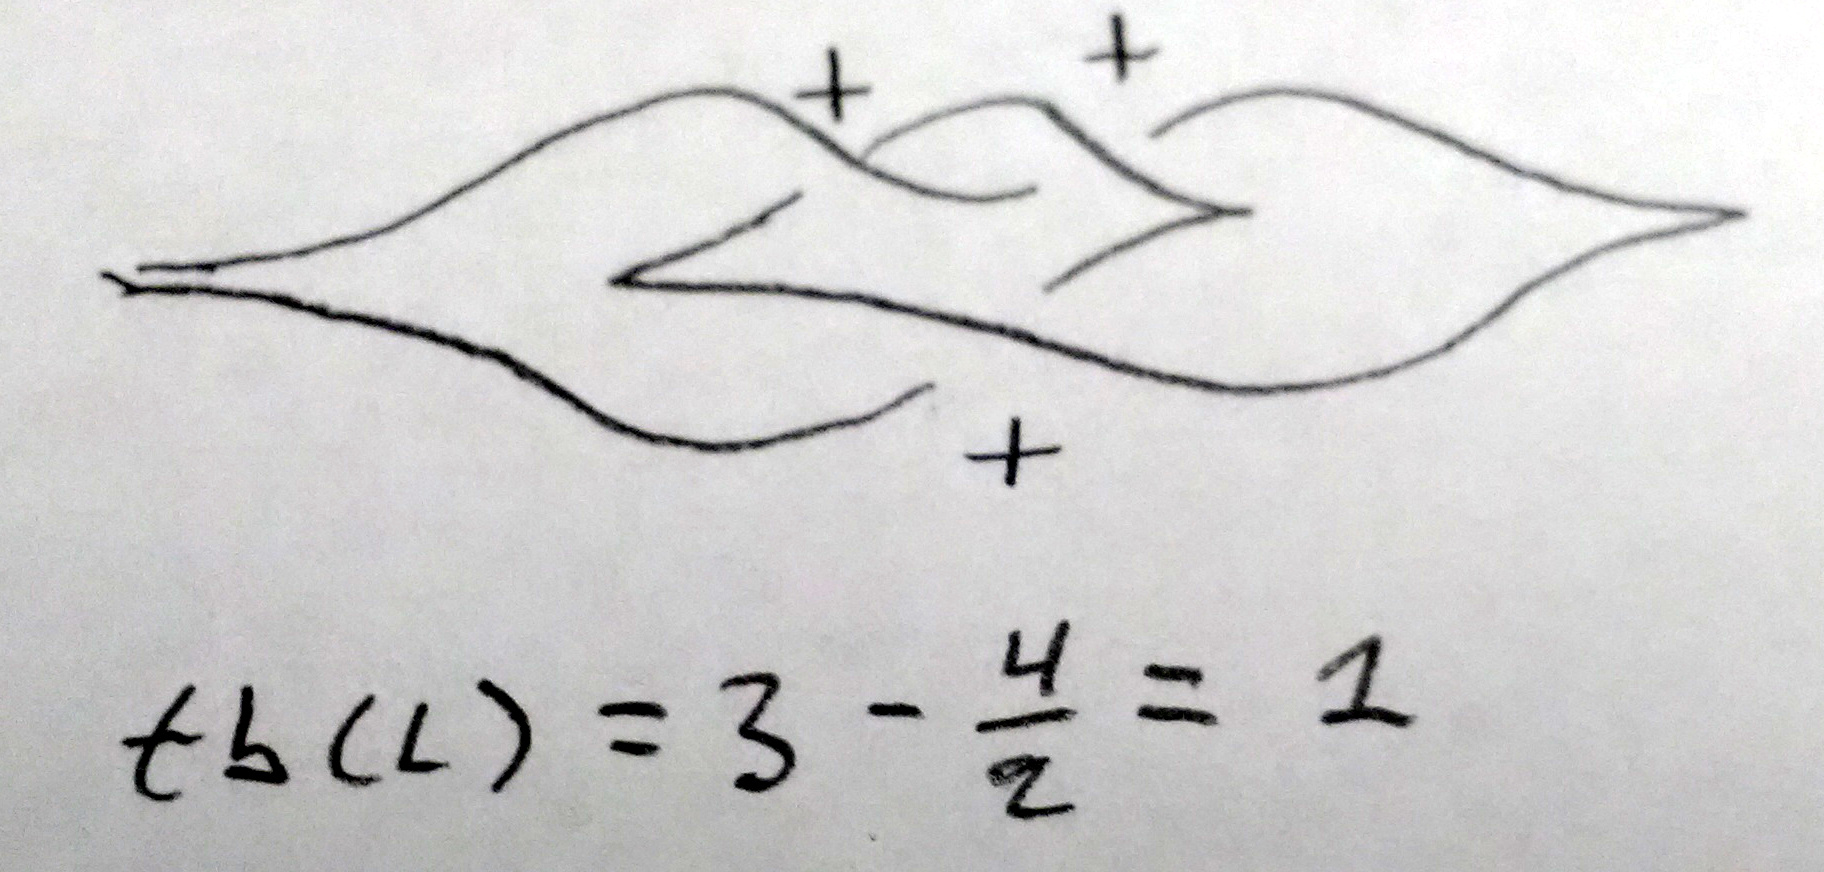
\includegraphics[height=3cm]{tbFront.jpg}
    \end{center}
\end{frame}

\begin{frame}
    \frametitle{Infinitely Many Non-equivalent Legendrian Knots}
    Given a front projection of $L$, we can always perform the following
    procedure to decrease its $tb$ number by 1:
    \begin{center}
    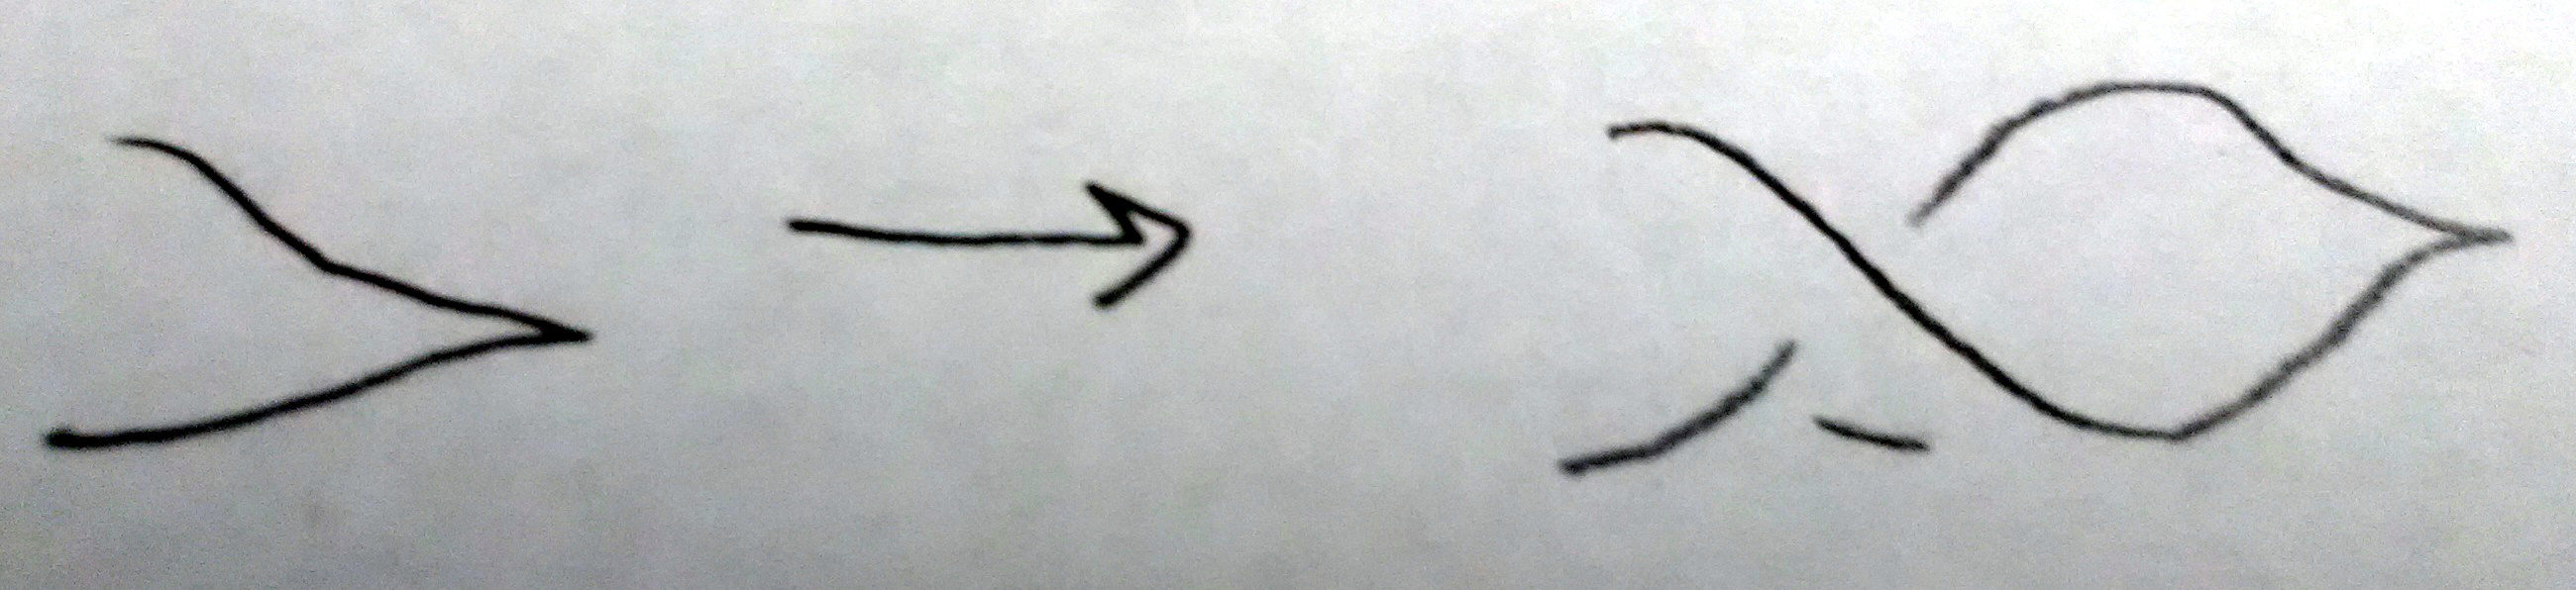
\includegraphics[height=2cm]{infKnots.jpg}
    \end{center}
    \begin{theorem}
    For any smooth knot $K$, there are infinitely many non-equivalent
    Legendrian knots with $K$ as their topological knot type.
    \end{theorem}
\end{frame}

\begin{frame}
    \frametitle{Calculating $tb(L)$ Using Lagrangian Projections}
    For a \textit{Lagrangian} projection, we need only the \textit{writhe}
    number of the projection. \\
    The formula is simply
    \[tb(L) = writhe(\pi(L)).\]
    \begin{center}
    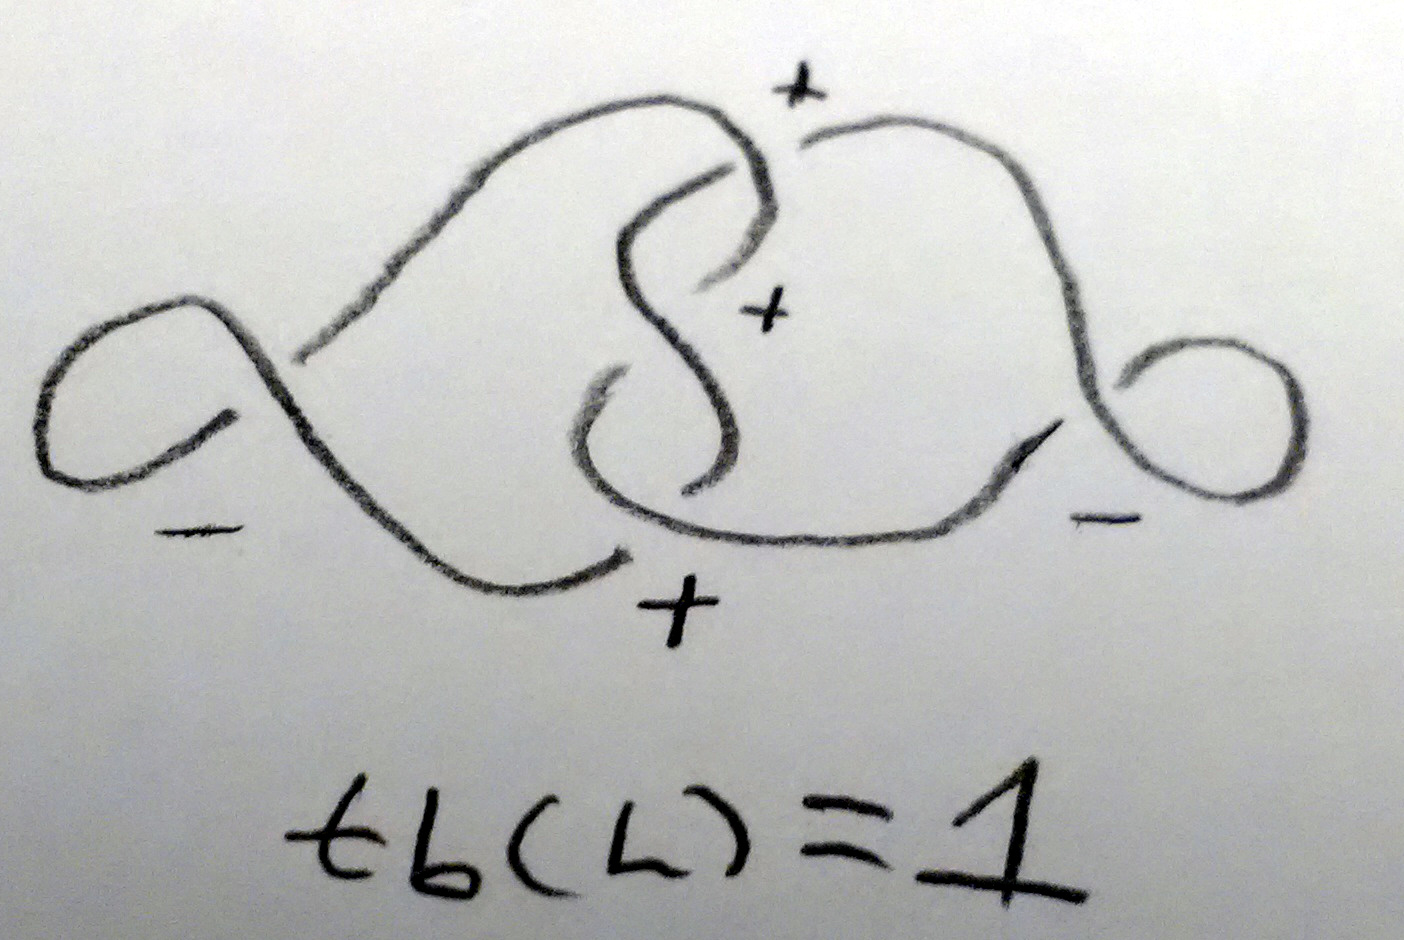
\includegraphics[height=4cm]{tbLagr.jpg}
    \end{center}
\end{frame}


\begin{frame}
    \frametitle{Rotation Number}
    The \alert{rotation number}, denoted \alert{$r(L)$}, of $L$ describes how
    much $L$ twists inside of the contact planes.
    Again, the geometric definition is elaborate, so we will describe the
    methods of effectively computing $r(L)$.
\end{frame}


\begin{frame}
    \frametitle{Calculating Rotation Number}
    With a \textit{front projection}:
    \begin{itemize}
        \item{We need the amount of \textit{down} cusps a projection has, denoted
        as \textit{D}.}
      \item{We also need the amount of \textit{up} cusps a projection has,
      denoted as \textit{U}.}
    \end{itemize}
    With this, our formula is:
    \[r(L) = \frac{1}{2}(D - U).\]
    \alert{NOTE}: Swapping the orientation will swap the sign of the rotation number,
    so $|r(L)|$ is the proper invariant for unoriented Legendrian knots.
\end{frame}

\begin{frame}
    \frametitle{Beyond the Classical Invariants}
    It turns out that these three invariants, $k(L)$, $tb(L)$, and $r(L)$
    are not sufficient to classify Legendrian knots. For example, these
    two Legendrian $5_2$ knots have the same $tb$ and $r$, and some very
    sophisticated tools are needed to tell them apart.

    \begin{center}
    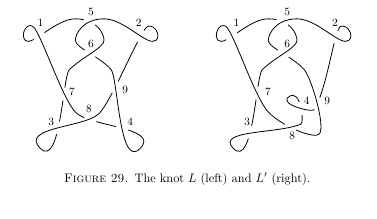
\includegraphics[height=5cm]{diffKnots.jpg}
    \end{center}
\end{frame}
\begin{frame}
    \frametitle{References}
    \begin{itemize}
        \item Sabloff, Joshua M (2009, November). \textit{What Is... a Legendrian Knot?}
        Notices of the AMS. Volume 56, Number 10.
    \end{itemize}
    \begin{itemize}
        \item Etnyre, John B (2005). \textit{Legendrian and Tranversal Knots.}
        Handbook of Knot Theory, Elsevier, pp. 105-185.
    \end{itemize}

\end{frame}

\end{document}
